\chapter{Metodología de evaluación}

\section{Entorno y escenarios}

La evaluación se planteó como un experimento controlado con dos máquinas
virtuales (VM) Linux aisladas en Google Cloud. En la VM de control se ejecutó
la carga sin el monitor; en la VM protegida se mantuvo activo Anti-Bunny Virus.
La unidad experimental es una corrida completa, desde la línea base hasta la
recuperación o finalización de la carga. Para una comparación directa, ambas
condiciones deben usar recursos equivalentes; las capturas disponibles no
permiten comprobar esa equivalencia en todos los parámetros.

\begin{table}[H]
  \centering
  \caption{Configuración documentada para la evaluación.}
  \label{tab:entorno-evaluacion}
  \small
  \begin{tabular}{p{0.28\textwidth}p{0.62\textwidth}}
    \toprule
    Elemento & Configuración \\
    \midrule
    Plataforma & Google Cloud, región \texttt{us-central1} (Iowa). \\
    VM de control & \texttt{vm1-sacrificable}: 2 vCPU, 4 GB de RAM y disco persistente de 10 GB en la pantalla de configuración. \\
    VM protegida & \texttt{vm2-protegida}: arquitectura x86-64 y disco de origen de 25 GB. \\
    Snapshot protegido & \texttt{snap-limpio}, instantánea estándar de 937,58 MB. \\
    Recursos en terminal & Las capturas de ejecución muestran 1,9 GiB utilizables y 0 B de \emph{swap}. \\
    Versión del software & Código de \texttt{main} (commit \texttt{a771cbc}), integrado en la rama del informe; verificado con \texttt{make check}. \\
    Muestreo del monitor & Un ciclo cada 0,25 s. \\
    Condición de control & Monitor inactivo y ejecución de la carga de procesos. \\
    Condición protegida & Monitor activo; modo \texttt{alerta} en la evidencia JSON. \\
    Identidad observada & Usuario \texttt{antibunny-test} y PGID 12480 en el JSON. \\
    Freno independiente & \texttt{PIDsMax=256} en la unidad protegida de \texttt{systemd}. \\
    Datos aún no consignados & Distribución, kernel, vCPU/RAM de la VM protegida y snapshot de la VM de control. \\
    \bottomrule
  \end{tabular}
\end{table}

\begin{figure}[H]
  \centering
  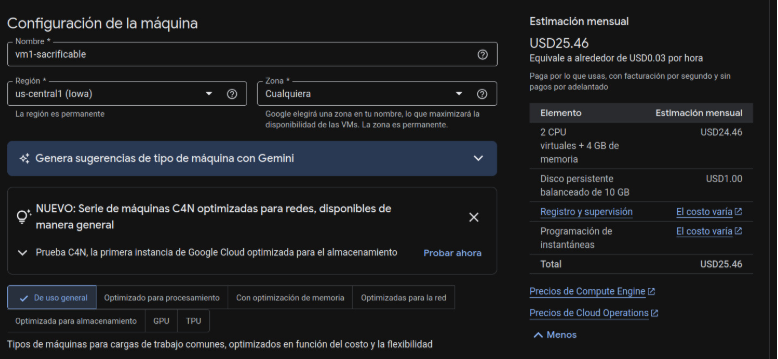
\includegraphics[width=0.95\textwidth]{figuras/metodologia/vm1_sacrificable.png}
  \caption{Configuración mostrada para la VM de control \texttt{vm1-sacrificable}.}
  \label{fig:vm1-configuracion}
\end{figure}

\begin{figure}[H]
  \centering
  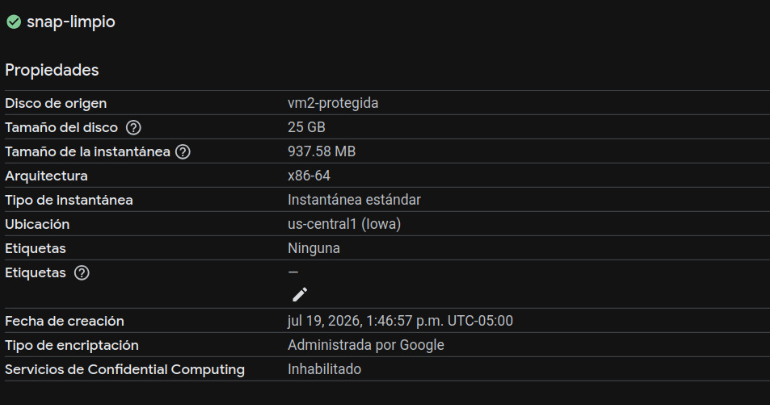
\includegraphics[width=0.95\textwidth]{figuras/metodologia/vm2_protegida_snapshot.png}
  \caption{Propiedades del snapshot \texttt{snap-limpio} asociado a \texttt{vm2-protegida}.}
  \label{fig:vm2-snapshot}
\end{figure}

Los campos no consignados en la Tabla~\ref{tab:entorno-evaluacion} no se
infirieron a partir de las Figuras~\ref{fig:vm1-configuracion} y
\ref{fig:vm2-snapshot}. Deben registrarse con
\texttt{scripts/validacion/preparar\_corrida.sh} antes de las repeticiones
finales. El diseño contempla tres repeticiones por condición. La evidencia
disponible en este informe es preliminar: incluye dos corridas sin protección
y una corrida con el monitor activo.

Los escenarios evaluables son línea base, proliferación de procesos, consumo
gradual de memoria y crecimiento de archivo. Para la comparación principal se
usa la misma carga de procesos en las VM de control y protegida. Los
simuladores de memoria y archivo se ejecutan por separado para evitar que sus
efectos se mezclen.

\section{Métricas}

Las métricas se obtienen de las capturas del recolector, el log JSON del
monitor, \texttt{/proc}, \texttt{free} y la salida del sistema. El instante de
inicio de la carga se denota por $t_0$; los tiempos de alerta y recuperación se
expresan respecto a ese instante.

\begin{table}[H]
  \centering
  \caption{Métricas y criterios de cálculo.}
  \label{tab:metricas-evaluacion}
  \small
  \begin{tabular}{p{0.25\textwidth}p{0.44\textwidth}p{0.20\textwidth}}
    \toprule
    Métrica & Cálculo & Fuente y unidad \\
    \midrule
    Alerta inicial & $t_{\mathrm{sospechosa}}-t_0$ & Log, segundos \\
    Alerta crítica & $t_{\mathrm{critica}}-t_0$ & Log, segundos \\
    Escalamiento & $t_{\mathrm{critica}}-t_{\mathrm{sospechosa}}$ & Log, segundos \\
    Pico de procesos & Máximo de procesos simultáneos & Recolector, procesos \\
    Procesos normalizados & $100N_{\mathrm{proc}}/N_{\mathrm{limite}}$ & Porcentaje \\
    Uso de RAM & $100M_{usada}/M_{asignada}$ & \texttt{free}, porcentaje \\
    Uso de CPU & Uso agregado dividido entre las vCPU asignadas & Porcentaje \\
    Recuperación & $t_{\mathrm{estable}}-t_{\mathrm{fin}}$ & Recolector, segundos \\
    Falsos positivos & Alertas críticas durante la línea base & Log, conteo \\
    Sobrecarga & Diferencia de CPU y RSS con y sin monitor & Porcentaje y MiB \\
    \bottomrule
  \end{tabular}
\end{table}

La mediana de las tres repeticiones será el valor representativo; el mínimo y
el máximo mostrarán la dispersión. Mientras no existan las tres corridas, se
reportan valores individuales y se identifican como preliminares. Los eventos
JSON se agrupan por marca temporal, severidad, PID y PGID. Una transición del
mismo PID desde \texttt{sospechosa} a \texttt{critica} representa persistencia,
no dos procesos diferentes.

\section{Procedimiento y medidas de seguridad}

Cada corrida sigue el mismo procedimiento:

\begin{enumerate}
  \item Restaurar el snapshot de la VM y comprobar RAM, vCPU, límite de PID,
        kernel y commit.
  \item Ejecutar \texttt{make check}, limpiar los logs de la corrida anterior
        e iniciar el recolector del sistema.
  \item Medir la línea base, registrar $t_0$ e iniciar una sola carga.
  \item En la VM protegida, iniciar primero Anti-Bunny Virus y comprobar el
        modo de respuesta, el usuario y el PGID autorizado.
  \item Registrar procesos, CPU, RAM, severidad, PID, PPID, PGID, ciclos y
        acciones hasta finalizar la carga y observar la recuperación.
  \item Copiar capturas y logs sin modificarlos, restaurar la VM y repetir el
        escenario tres veces.
\end{enumerate}

Las pruebas se limitan a VM aisladas, con consola disponible y usuario de
laboratorio sin privilegios. La unidad protegida aplica
\texttt{PIDsMax=256} como freno independiente. La contención solo puede
habilitarse en modo \texttt{terminar\_lab}, para un PGID publicado y un usuario
autorizado; en los demás casos el sistema únicamente alerta. No deben
ejecutarse cargas ilimitadas en el equipo anfitrión. Si la VM deja de responder,
se detiene la corrida desde el hipervisor y se restaura el snapshot.

El análisis conserva por separado los datos crudos y los datos derivados. El
archivo \texttt{informe/datos/anti\_bunny\_virus\_logs.json} es la fuente de la
tabla y la gráfica del sistema protegido; así se mantiene la trazabilidad entre
cada resultado y el evento original.
